% Report
\documentclass{article}

% Here set the various packages
% Packages to load
\usepackage[english]{babel}
% %%% Support some german text
% \usepackage{ngerman}
% \usepackage[latin1]{inputenc}   % für Umlaute
%%%
% \usepackage[utf8]{inputenc}
\usepackage[T1]{fontenc}
\usepackage{microtype}

%%%
% \usepackage[inline]{enumitem} % Required for the "description" list.

%%% Fix for not hyperlinking citations
\makeatletter
\let\NAT@parse\undefined
\makeatother
\usepackage{hyperref}
% 
\usepackage{cite}
% \ifx\pdfoutput\undefined
% 	\usepackage{graphicx}
% \else
% 	\usepackage[pdftex]{graphicx}
% \fi
\usepackage{graphicx}
\graphicspath{{Figures/}}
\usepackage{amsmath}
% \interdisplaylinepenalty=2500

% Shading of questions. Use the "shaded" environment or the "\hl{}" command.
\usepackage{framed}
% \usepackage[dvipsnames]{color}
\usepackage[svgnames]{xcolor}
\usepackage{soul}
% Nice colours: Gainsboro, LightGoldenrod, LightSteelBlue
% furter ref: https://www.latextemplates.com/svgnames-colors
\definecolor{shadecolor}{named}{Gainsboro}
\sethlcolor{Gainsboro}

%%% Todo margin notes (enable/disable)
\usepackage{todonotes}
% \usepackage[disable]{todonotes}
%%%

%eof

%%%

\title{Programming of Supercomputers\\Worksheet 2}
\author{Oleksandr Voloshyn\\ Qunsheng Huang\\ Tommaso Bianucci}
\date{\today}

\begin{document}

\maketitle
\renewcommand{\abstractname}{Group members's contributions}
\begin{abstract}
	% Here write the contributions of the members of the group
	Here briefly state the contributions of the different members of the group!
\end{abstract}

\section{Task 1}
\subsection{Concepts description}
\begin{description}
	\item[Race condition] www
	\item[Deadlock] www
	\item[Heisenbug] www
	\item[Cache coherency and false sharing] www
	\item[Load imbalance] www
	\item[Amdahl's law] www
	\item[Parallelization overhead] www
	\item[Floating-point arithmetic challenges] ~

		\begin{description}
			\item[Comparisons] www
			\item[Definition of zero and signed zero] www
			\item[Cancellation or loss of significance] www
			\item[Amplificatio and error propagation] www
		\end{description}
\end{description}

\subsection{Questions}
\begin{enumerate}
	\item \hl{Which of the concepts affect performance but not correctness?}

	www

	\item \hl{Which of the concepts affect the correctness of the application?} ~

	\begin{enumerate}[label=\Alph*]
		\item \hl{Of these, which are exclusive to parallel programming?}

		www

		\item \hl{Of these, which are not exclusive to parallel programming?}

		www
	\end{enumerate}

	\item \hl{Which of them can occur in OpenMP applications?}

	www
	
	\item \hl{Which of them can occur in MPI applications?}

	www
	
	\item \hl{Is cache coherency necessary on MPI applications with a single process and a single thread per rank? Explain.}

	www
	
	\item \hl{Is Amdahl's law applicable to strong scaling applications? Explain.}

	www
	
	\item \hl{Is Amdahl's law applicable to weak scaling applications? Explain.}

	www
	
	\item \hl{Which of these limit the scalability of applications?}

	www
	
\end{enumerate}

% Figure example
\begin{figure}[h!] % h=here, t=top, b=bottom, p=(extra)page, !=force
 	\begin{center}
 		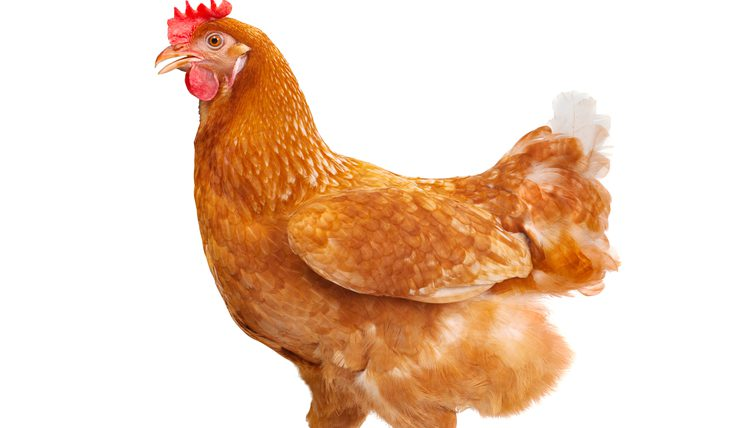
\includegraphics[width=.9\linewidth]{figure.png} % It searches in the Figures/ folder!
 		\caption{Caption text}
 		\label{fig:figureLabelName}
 	\end{center}
\end{figure}

\section{Name of assignment 2}
\subsection{Name of sub-assignment 2.1}
Lorem ipsum

\end{document}

%eof
